\chapter{Quantum Chromodynamics}


The U(1)-gauge-invariant QED Lagrangian consists of the gauge part and the matter part:
\begin{equation}
\begin{aligned}
	\mathcal L_{\mathrm{QED}} &= \mathcal L_\gamma + \mathcal L_\psi \\
	&= -\frac{1}{4} F^{\mu\nu} F_{\mu\nu} + \bar\psi(i\cancel D-m)\psi.
\end{aligned}
\end{equation}
where the gauge-covariant derivative 
\begin{equation}
	D_\mu = \partial_\mu - iq A_\mu
\end{equation}
and the field strength tensor
\begin{equation}
	F_{\mu\nu} = \frac{i}{q} [D_\mu, D_\nu] = \partial_\mu A_\nu -\partial_\nu A_\mu
\end{equation}
are all manifestly invariant under U(1) gauge transformation.

The nonabelian gauge theory generalize the gauge group to be a general (nonabelian) Lie group parametrized as
\begin{equation}
	U(x) = \exp\left[-i g \pi^a(x) T^a\right],
\end{equation}
where $\{T^a\}$ are the generators of the gauge group.
For the nonabelian Lie group, the commutation relation, the Lie algebra, specify the structure of the infinitesimal gauge transformation.

\section{Yang-Mills Theory}
The gauge-invariant Lagrangian can be:
\begin{equation}
\begin{aligned}
	\mathcal L_{\mathrm{n.a.}} &= \mathcal L_{\mathrm{YM}} + \mathcal L_{\mathrm{matter}} \\
	&= -\frac{1}{4} F^{a,\mu\nu} F^a_{\mu\nu} + \bar\psi(i\cancel D-m)\psi.
\end{aligned}
\end{equation}
The form of Yang-Mills Lagrangian similar to the Maxwell field:
\begin{equation}
	\mathcal L_{\mathrm{YM}} = -\frac{1}{4} F^{a,\mu\nu} F^a_{\mu\nu}.
\end{equation}
To get gauge-invariant Lagrangian for the matter fields, we simply replace the ordinary derivative with the gauge-covariant derivative:
\begin{equation}
	\mathcal L_{\mathrm{matter}} = \begin{cases}
		\psi(i\gamma^\mu D_\mu - m)\psi & \text{Fermion} \\
		(D^\mu \phi)^\dagger D_\mu \phi - m^2 \phi^\dagger \phi & \text{Scalar}
	\end{cases}.
\end{equation}
The covariant derivative $D_\mu$ is now defined as
\begin{equation}
	D_\mu = \partial_\mu - i g A_\mu^a T^a,
\end{equation}
and the field-strength tensor is then
\begin{equation}
\begin{aligned}
	F^a_{\mu\nu} &= \frac{i}{g}[D_\mu, D_\nu]^a \\
	&= \partial_\mu A_\nu^a - \partial_\nu A_\nu^a -ig f^{abc} A^b_\mu A^c_\nu,
\end{aligned}
\end{equation}
The field strength tensor $F_{\mu\nu}$ transform as
\begin{equation}
	F_{\mu\nu}(x) \rightarrow U(x) F_{\mu\nu}(x) U^\dagger(x).
\end{equation}
The Lagrangian 
\begin{equation*}
	\mathcal L_{\mathrm{GI}} = -\frac{1}{2} \mathrm{Tr}\left[F_{\mu\nu} F^{\mu\nu}\right]
\end{equation*}
is manifestly gauge-invariant.
Also, we can also choose the renormalization of the generators so that $\mathrm{Tr}[T^aT^b] = \delta^{ab}$.
In this way, when express the field strength as $F_{\mu\nu} = F_{\mu\nu}^a T^a$, the above gauge-invariant Lagrangian is exactly the Yang-Mills Lagrangian $\mathcal L_{\mathrm{YM}}$.

The covariant derivative transforms as
\begin{equation}
	D_\mu \rightarrow U(x) D_\mu U^\dagger(x)
	=\partial_\mu - i g \left[U(x) A_\mu(x) U^\dagger(x) + \frac{i}{g} U(x)\partial_\mu U^\dagger(x)\right].
\end{equation}
The matter part $\mathcal L_{\mathrm{matter}}$ is invariant if we define the transformation of the gauge field as:
\begin{equation}\label{eq:SM-YM-GT-1}
	A_\mu(x) \rightarrow U(x) A_\mu(x) U^\dagger(x) + \frac{i}{g} U(x)\partial_\mu U^\dagger(x).
\end{equation}



\subsection{Faddeev-Popov Quantization}
Similar to QED case, the gauge redundancy causes trouble in quantization.
We follow the Faddeev-Popov procedure to quantize the Yang-Mills Lagrangian.

The partition function of the Yang-Mills Lagriangian is
\begin{equation}
	Z = \int D[A] \exp\left(i \int d^4x \mathcal{L}[A]\right)
	= \int D[A_{f}]\ \mathcal V_G[A] \exp\left(i \int d^4x \mathcal{L}_{\mathrm{YM}}[A_f]\right)
\end{equation}
where $A_f$ is the gauge-fixed field, and $\mathcal V_G[A]$ denotes the phase volume of the gauge redundancy.
The task is to determine $\mathcal V_G[A]$. 
This can be done by introducing a gauge-fixing condition:
\begin{equation}
	Z = \int D[\pi] \mathcal V_G[A]\int D[A] \delta(G[A^\pi]) \exp\left(i \int d^4x \mathcal{L}_{\mathrm{YM}}[A^\pi]\right),
\end{equation}
where the gauge-fixing function is 
\begin{equation}\label{eq:SM-YM-GF-1}
	G[A] = \partial^\mu A_\mu - X.
\end{equation}
Here $D[\pi]$ is the Haar measure over the Lie group.
$A^\pi$ denotes the gauge transformed field. 
Since the Lagrangian is gauge-invariant, we can simply drop a superscript, and the integral over $\pi$ field is just a number depending on $A$:
\begin{equation}
	\int D[\pi] \delta(G[A]) = \det\left(\frac{\delta G[A^\pi]}{\delta \pi}\right)^{-1}
\end{equation}
The infinitesimal version of the gauge transformation (\ref{eq:SM-YM-GT-1}) is
\begin{equation}
	A_\mu^a \rightarrow A_\mu^a +\frac{1}{g}\partial_\mu \pi^a + f^{abc}A^b_\mu \pi^b
	\equiv A_\mu + \frac{1}{g} D_\mu \pi^a,
\end{equation}
where the covariant derivative on the operator involves the adjoint representation:
\begin{equation}
	D_\mu \pi^a = \partial_\mu \pi^a + g f^{abc} A_\mu^b \pi^c = \partial_\mu -i g A_\mu^a \left(T^a_{\mathrm{adj}}\right)_{bc} \pi^c.
\end{equation}
The integral is then formally the operator determinant, and we thus know
\begin{equation}
	 \mathcal V_G[A] = \det(\partial^\mu D_\mu).
\end{equation}
This functional determinant can be regarded as the functional integral on a ``ghost'' field:
\begin{equation}
	\det(\partial^\mu D_\mu) = \int D[\bar c,c] \exp\left[i \int d^4 x\ \bar c (-\partial^\mu D_\mu)c \right].
\end{equation}
The gauge-fixing condition (\ref{eq:SM-YM-GF-1}) impose a hard constraint on the field configuration.
For our convenience, we 
\begin{equation}
\begin{aligned}
	Z &= \int DX e^{-\frac{X}{2 \xi}}\int D[A_X] \exp\left\{i\int d^4x \left[\mathcal{L}_{\mathrm{YM}} - \bar c\partial^\mu D_\mu c \right]\right\} \\
	&= \int D[A] e^{-\frac{i}{2\xi}(\partial^\mu A_\mu)^2} \exp\left\{i\int d^4x \left[\mathcal{L}_{\mathrm{YM}} -\frac{1}{2\xi}(\partial^\mu A_\mu)^2 - \bar c\partial^\mu D_\mu c \right]\right\}.
\end{aligned}
\end{equation}
The gauge-fixing results in a modified Lagrangian with gauge-fixing term and ghost term:
\begin{equation}
\begin{aligned}
	\mathcal L &= \mathcal{L}_{\mathrm{YM}} + \mathcal{L}_{\mathrm{gf}} + \mathcal{L}_{\mathrm{gh}}, \\
	\mathcal{L}_{\mathrm{gf}} &= -\frac{1}{2\xi}(\partial^\mu A_\mu)^2, \\
	\mathcal{L}_{\mathrm{gh}} &= -\bar c\partial^\mu D_\mu c.
\end{aligned}
\end{equation}

In the standard model, the weak and strong interaction is described by the SU(2) and SU(3) Yang-Mills theory respectively, so we mainly focus on the those two cases.


\subsection{Feynman Rules}

The SU(3) Yang-Mills theory describe the strong interaction, also known as the quantum chromodynamics (QCD).
The Feynman rule in QCD is very complicated.
Here we just consider the simplest tree-level process $u \bar d \rightarrow u \bar d$, corresponding to the diagram
\begin{equation}
	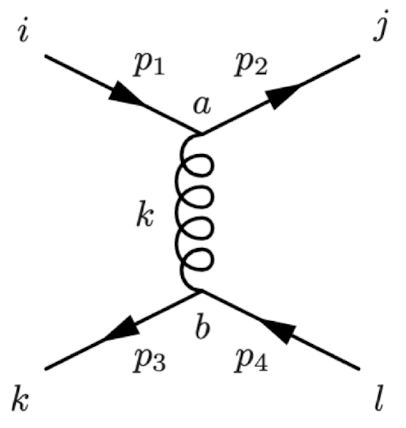
\includegraphics[width=0.2\linewidth,align=c]{pics/SM-YM-1}
	= T^a_{ji} T^a_{kl} \times (\text{QED-like term}),
\end{equation}
where the index $i$ labels the color:
\begin{equation}
	\begin{tabular}{c c c}
		\hline
		Index & Color & Simbol \\ \hline
		1 & red & $r$ \\ 
		2 & green & $g$ \\  
		3 & yellow & $y$ \\
		\hline
	\end{tabular}
\end{equation}
Since the total color is conserved in the scattering process, we can divide the color degrees of freedom to the singlet and octet, corresponding to
\begin{equation}
	3\otimes \bar 3 = 1 \otimes 8.
\end{equation}
The singlet states is
\begin{equation}
	|s\rangle = \frac{1}{\sqrt 3} \left(|r\bar r\rangle + |g\bar g\rangle + |y\bar y\rangle\right)
\end{equation}
The factor then becomes
\begin{equation}
	\left(\frac{1}{\sqrt{3}} \right)^2 (T^aT^a)_{jl} = \frac{4}{9} \delta_{jl}.
\end{equation}
For the octet state $|r \bar y\rangle$
\begin{equation}
	T^a_{i1} T^a_{3l} = -\frac{1}{6} \delta_{i1}\delta_{l3}.
\end{equation}
In QED, we know that two particle with opposite charge are attractive to each other.
From the factors above, we know that color singlet channel is attractive while the color octet channel is repulsive.
Indeed, in QCD there is phenomenon named \textit{color confinement}, which means quarks tend to form composite colorless bound state.


\subsection{Lattice QCD}



\section{SU(3) Lie Algebra}
For the fundamental representation, the generators for the SU(3) is one-half of the \textit{Gell-Mann matrices} $T^a = \frac{1}{2}\lambda^a$, $a=1,\dots,8$, where the 8 matrices are:
\begin{equation}
\begin{aligned}
	\lambda^1 &= \left[\begin{array}{ccc}
		0 & 1 & 0 \\ 1 & 0 & 0 \\ 0 & 0 & 0
	\end{array} \right], &
	\lambda^2 &= \left[\begin{array}{ccc}
		0 & -i & 0 \\ i & 0 & 0 \\ 0 & 0 & 0
	\end{array} \right], \\
	\lambda^3 &= \left[\begin{array}{ccc}
		1 & 0 & 0 \\ 0 & -1 & 0 \\ 0 & 0 & 0
	\end{array} \right], &
	\lambda^4 &= \left[\begin{array}{ccc}
		0 & 0 & 1 \\ 0 & 0 & 0 \\ 1 & 0 & 0
	\end{array} \right], \\
	\lambda^5 &= \left[\begin{array}{ccc}
		0 & 0 & -i \\ 0 & 0 & 0 \\ i & 0 & 0
	\end{array} \right], &
	\lambda^6 &= \left[\begin{array}{ccc}
		0 & 0 & 0 \\ 0 & 0 & 1 \\ 0 & 1 & 0
	\end{array} \right], \\
	\lambda^7 &= \left[\begin{array}{ccc}
		0 & 0 & 0 \\ 0 & 0 & -i \\ 0 & i & 0
	\end{array} \right], &
	\lambda^8 &= \frac{1}{\sqrt{3}}\left[\begin{array}{ccc}
		1 & 0 & 0 \\ 0 & 1 & 0 \\ 0 & 0 & -2
	\end{array} \right].
\end{aligned}
\end{equation}
The commutation relation among the generator defines the \textit{structure constant}:
\begin{equation}
	\left[T^a, T^b\right] = i f^{abc} T^c.
\end{equation}
The product of two SU(3) generators is
\begin{equation}
	T^a T^b = \frac{1}{6}\delta^{ab} + \frac{1}{2} d^{abc} T^c + \frac{i}{2} f^{abc} T^c,
\end{equation}
where
\begin{equation}
	\frac{i}{2} f^{abc} = \mathrm{Tr}\left([T^a,T^b]T^c \right), \quad
	\frac{1}{2} d^{abc} = \mathrm{Tr}\left(\{T^a,T^b\}T^c \right).
\end{equation}
The cycling properties of the trace expression leads to 
\begin{equation}
	f^{abc} = f^{bca} = f^{cab}, \quad
	d^{abc} = d^{bca} = d^{cab}.
\end{equation}
It also manifest that $f^{abc}$ is totally anti-symmetric and $d^{abc}$ totally symmetric.
This also leads to the trace identities:
\begin{equation}
\begin{aligned}
	\mathrm{Tr}(T^a T^b) &= \frac{1}{2}\delta^{ab}, \\
	\mathrm{Tr}(T^a T^b T^c) &= \frac{1}{4}(d^{abc} + if^{abc}), \\
	\mathrm{Tr}(T^a T^b T^c T^d) &= \frac{1}{12} \delta^{ab}\delta^{cd} + \frac{1}{8}(d^{abe}+if^{abe})(d^{cde}+if^{cde}).
\end{aligned}
\end{equation}

The generator in representation labeled by $R$ is denoted as $T_R^a$.
One important representation apart from the fundamental representation is the adjoint representation, which is a 8-dimensional representation defined as
\begin{equation}
	(T^a_{\mathrm{adj}})^{bc} = -i f^{abc}.
\end{equation}

Also, different representations can be characterized by the quadratic Casimir $C_2(R)$ defined as
\begin{equation}
	T^a_R T^a_R = C_2(R) \mathbbm 1.
\end{equation}
We know
\begin{equation}
	C_2(\text{fund}) = \frac{4}{3},\quad
	C_2(\text{adj}) =3.
\end{equation}
This also means
\begin{equation}
	f^{acd} f^{bcd} = 3 \delta^{ab}.
\end{equation}





\subsection{Roots and Weights}
For a simple Lie algebra, a standard set of generators (called the \textit{Cartan-Weyl basis}) can be chosen so that it contains a maximal number of mutually commuting subset.
The maximum number of such generators is defined as the \textit{rank} of the algebra.
The SU(3) Lie algebra is rank-2, with the Cartan-Weyl basis
\begin{equation}
	H_1 = \frac{1}{2}\lambda_3, \quad H_2 = \frac{1}{2}\lambda_8
\end{equation}
The common eigenstates of Cartan sub-algebra is denoted as $\{|\bm m\rangle\}$, where each $\bm m$ is a vector, called the \textit{weight}, defined by
\begin{equation}
	H_i |\bm m\rangle = m_i |\bm m\rangle.
\end{equation}
Apart from the Cartan sub-algebra, other generators can be linearly combined to form a standard non-Hermitian basis $\{E^\pm_{\bm \alpha}\}$.
Each element is labeled by an $r$-dimensional vectors $\pm \bm\alpha$, called the \textit{root}, which is defined by the commutation relation:
\begin{equation}
	[H_i, E_{\bm \alpha}^\pm] = \pm \alpha_i E^\pm_{\bm \alpha}.
\end{equation}
We can also denote $E_{\pm\bm{\alpha}} \equiv E_{\bm{\alpha}}^\pm$ for notational simplicity.
Note that the action of $E_\alpha$ will change the weight,
\begin{equation}
\begin{aligned}
	H_i E_{\bm \alpha}|\bm m\rangle 
	&= [H_i, E_{\bm \alpha}]|\bm m\rangle + E_{\bm \alpha} H_i |\bm m\rangle \\
	&= (m_i + \alpha_i) E_{\bm \alpha}|\bm m\rangle,
\end{aligned}
\end{equation}

For SU(3), since $\{H_i\}$ are all diagonal, the common eigenstates are
\begin{equation}
	\begin{bmatrix}
		1 \\ 0 \\ 0
	\end{bmatrix} = \left|\left(\frac{1}{2}, \frac{\sqrt{3}}{6}\right)\right\rangle, \quad
	\begin{bmatrix}
		0 \\ 1 \\ 0
	\end{bmatrix} = \left|\left(-\frac{1}{2}, \frac{\sqrt{3}}{6}\right)\right\rangle, \quad
	\begin{bmatrix}
		0 \\ 0 \\ 1
	\end{bmatrix} = \left|\left(0, -\frac{\sqrt{3}}{3}\right)\right\rangle.
\end{equation}
These vectors, plotted in a plane, form a equilateral triangle:
\begin{equation}
	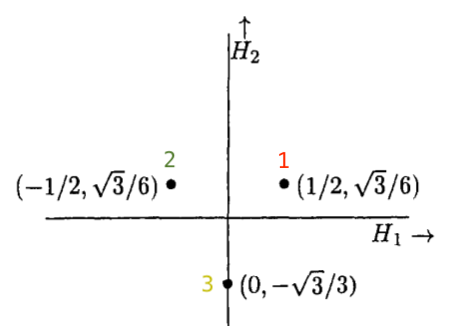
\includegraphics[width=0.35\linewidth,align=c]{pics/SM-LA-SU3-1.png}
\end{equation}
Other generators are labeled by 
\begin{equation}
	E_{\bm{\alpha}_1} = \left[\begin{array}{ccc}
		0 & 1 & 0 \\ 0 & 0 & 0 \\ 0 & 0 & 0
	\end{array}\right], \quad
	E_{\bm{\alpha}_2} = \left[\begin{array}{ccc}
		0 & 0 & 0 \\ 0 & 0 & 1 \\ 0 & 0 & 0
	\end{array}\right], \quad
	E_{\bm{\alpha}_3} = \left[\begin{array}{ccc}
		0 & 0 & 1 \\ 0 & 0 & 0 \\ 0 & 0 & 0
	\end{array}\right],
\end{equation}
where the root vectors are
\begin{equation}
	\bm{\alpha}_1 = (1, 0), \quad  
	\bm{\alpha}_2 = \left(-\frac{1}{2}, \frac{\sqrt 3}{2} \right), \quad
	\bm{\alpha}_3 = \left(\frac{1}{2}, \frac{\sqrt 3}{2} \right).
\end{equation}
The root vectors plotted in a plane form a regular hexagon:
\begin{equation}
	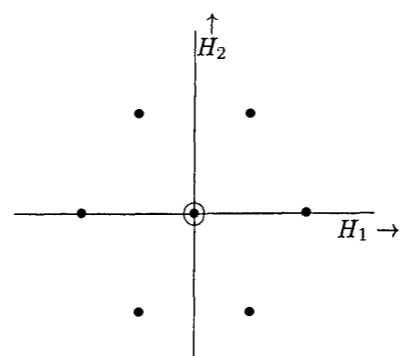
\includegraphics[width=0.35\linewidth,align=c]{pics/SM-LA-SU3-2.png}
\end{equation}

The roots of $\mathfrak{su}(3)$ are not linearly independent.
We can find a set of linear independent roots called the \textit{simple roots}.
All other roots can be expressed as a linear combination of simples roots with all positive/negative coefficients. 
The SU(3) algebra, for example, has $\bm{\alpha}_1$ and $\bm{\alpha}_2$ as its simple roots.



\subsection{Irreducible Representations}

An irreducible representation (Irrep) of a Lie algebra is entirely specified by the \textit{highest weight} state $|\bm M\rangle$ in the Irrep, which satisfies
\begin{equation}
	E_{\bm \alpha}|\bm M\rangle = 0
\end{equation}
for all simple root.
The Irrep then can be constructing by applying the lowering operators to the highest weight state:
\begin{equation}
	\text{Irrep} = \mathrm{span}\left\{ E_{\bm \alpha}^- E_{\bm \beta}^- \cdots E_{\bm \gamma}^- |\bm M\rangle, \ \text{all possible sequence}\right\}.
\end{equation}

The highest weight state can be systematically constructed using the tensor method.
For SU(3), we first need to introduce the complex of the fundamental representation $\bar 3$, defined by
\begin{equation}
	\exp(-i \pi^a T_{\bar 3}^a) = \exp(-i \pi^a T_{3}^a)^*,
\end{equation}
which gives
\begin{equation}
	T_{\bar 3}^a = - (T_{3}^{a})^T.
\end{equation}
The definition flip the sign of $\{H_i\}$, the weight plotted in the plane becomes the upside-down triangle:
\begin{equation}
	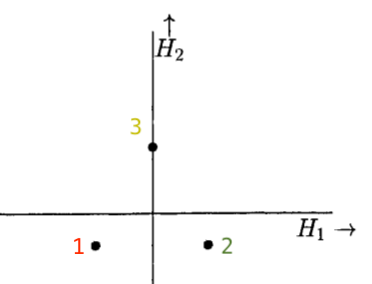
\includegraphics[width=0.35\linewidth,align=c]{pics/SM-LA-SU3-3.png}
\end{equation}
The highest wight state in $\bar 3$ is $|3\rangle$.
For a general Irrep (which can be labeled by ($m,n$)-representation), the highest weight states is
\begin{equation}
	|\bm M\rangle = \bigotimes_{i=1}^m |1\rangle_i \bigotimes_{j=m+1}^{m+n} |3\rangle_j.
\end{equation}
The ladder operators are now
\begin{equation}
	E_{\bm \alpha} = \sum_{i=1}^m E_{\bm \alpha}^{(i)} - \sum_{j=m+1}^{m+n} E^{(j)}_{-\bm \alpha}.
\end{equation}
The adjoint representation of the SU(3) is the $(1,1)$-representation. 






